
% Setting all the margins and boxes
\newgeometry{
letterpaper,
top=1.5cm,
bottom=1.4cm,
footskip=0.1cm,
inner=2.5cm,
outer=1cm,
marginparwidth=0cm
}
\setlength{\columnsep}{30pt}

\changefontsize{13pt}

% Positioning page-numbers
\pagestyle{fancy}
\fancyhf{}
\fancyfoot[L]{\llap{\textbf{50}}} % \llap to move the number "out of bounds"
\renewcommand{\headrulewidth}{0pt} % Because of fancyhdr, a line appears at the top of the page

\begin{multicols}{2}
\noindent
под силу многим поступающим. Все догадываются возвести обе его части в квадрат и получить квадратное уравнение с корнями $y_{1,2} = \dfrac{3 \pm \sqrt{5}}{2}$, но затем выявляются разные \guillements{точки зрения}; одни вообще не думают о том, что при таком решении могут появиться посторонние корни; другие знают, почему, и, как правило, уверены, что посторонними будут те корни, которые не входят в ОДЗ (область допустимых значений); третьи пытаются проверить корни непосредственной подстановкой их в уравнение - этот способ в принципе правилен, но удобен лишь для проверки \guillements{хороших} корней, а $y_1$ и $y_2$ не очень \guillements{хороши}.

Однако совершенно очевидно, что поскольку левая часть в уравнении (*) неотрицательна, то из чисел $y_1$ и $y_2$ корнем будет лишь то, для которого неотрицательна и правая часть. Поэтому единственным корнем уравнения (*) является $y = \dfrac{3 + \sqrt{5}}{2}$, и для нахождения $x$ мы получаем уравнение $\log_x 2 = \dfrac{-(9 + \sqrt{5})}{2}$.

Подчеркнем: при решении мы полностью обошлись без нахождения ОДЗ исходного уравнения. Между тем в последнее время среди абитуриентов широко распространился предрассудок, что решение любого уравнения или неравенства нужно обязательно начинать с вычисления ОДЗ. Такое мнение, однако, не имеет никаких теоретических оснований, а на практике оказывает плохую услугу: те, кто пошел по этому пути, должны были решать не только данное уравнение, но и придуманное ими самими логарифмическое неравенство $-1 - \log_x{2x^2} \geq 0$ - задачу, не менее сложную. Вообще, не строго определенного правила, надо или не надо в начале решения находить ОДЗ, и уже здесь, при выборе пути, поступающий может показать, насколько он умеет мыслить конкретно и самостоятельно.

\setcounter{taskcounter}{2}
\task Данное неравенство мы не будем решать подробно. Раскрыв скобки, мы легко приведем к квадратному неравенству относительно $x$:

\centerline{$2\sin^{2}{x} + 4 \sqrt{2} \sin{x} + 3 > 0,$}

\noindent
решив которое мы получим простейшее тригонометрическое неравенство $\sin{x} > - \tfrac{\sqrt{2}}{2}$. Но... именно с ним и не справилось большинство абитуриентов. Мы не будем анализировать данные ими ответы, часто совершенно бессмысленные, и просто обращаем внимание будущих абитуриентов на такие задачи. Способ решения достаточно ясно описан и в учебнике, и во многих пособиях, и надо только сознательно его усвоить. Заметим еще, что даже те, кто правильно решил простейшее неравенство, не всегда вспоминали, что из полученных решений, не всегда вспоминали, что из полученных решений надо выбросить значения $x$, при которых не имеет смысла $\tg{x}$.

\task Оказалась слишком \guillements{коварной} для тех абитуриентов, кто привык решать задачи только на правильные геометрические тела. Они не смогли отказаться от шаблонов и ошибочно представляли себе данную геометрическую конфигурацию. Так, очень многие считали \guillements{по привычке}, что высотой в $\triangle BKD$ является отрезок $KO$ (рис. \ref{fig:70-triangle}).

Но ведь каждому известно, что геометрическое воображение является лишь вспомогательным средством решения задач, и факты, \guillements{увиденные} на чертеже, требуются еще строго до-

\begin{figure}[H]
    \hfill % Using horizontal filling because `right` argument for graphics doesn't work
    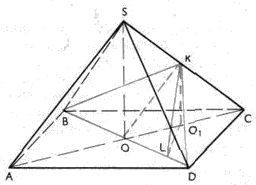
\includegraphics[width=.4\textwidth]{kvant_70-triangle-transparent.png}
    \caption{{}}
    \label{fig:70-triangle}
\end{figure}

\end{multicols}